\documentclass[border=3pt]{standalone}
% Preâmbulo compartilhado pelos diagramas TikZ da aula 7 (Filtros Não Paramétricos)
\usepackage[T1]{fontenc}
\usepackage[utf8]{inputenc}
\usepackage{lmodern}
\usepackage{amsmath}
\usepackage{xcolor}
\usepackage{tikz}
\usetikzlibrary{arrows.meta,angles,quotes,decorations.pathmorphing,calc,
                positioning,shapes.geometric,shapes.misc,backgrounds,fit,
                math}

% Paleta (mesma dos SVGs originais)
\definecolor{dblue}{HTML}{2A5B8C}
\definecolor{dorange}{HTML}{B3541E}
\definecolor{dgreen}{HTML}{4A7C59}
\definecolor{dred}{HTML}{9C4B4B}
\definecolor{dcream}{HTML}{F4F1EA}
\definecolor{dshade}{HTML}{DDD7C9}

% Função gaussiana (não normalizada por padrão de escala visual)
\pgfmathdeclarefunction{gauss}{3}{%
  \pgfmathparse{1/(#3*sqrt(2*pi))*exp(-((#1-#2)^2)/(2*#3^2))}%
}

% Estilos comuns (prefixo d... para não colidir com chaves internas do pgf)
\tikzset{
  >={Stealth[length=2mm]},
  dguide/.style={gray!55, dashed, line width=0.4pt},
  daxis/.style={gray!60, line width=0.7pt, ->},
  dbody/.style={fill=black!3, draw=black!80, line width=1pt},
  dacc/.style={draw=dblue, line width=1pt},
  dlbl/.style={black!55, font=\small},
  dsub/.style={black!45, font=\footnotesize},
  dstate/.style={circle, draw=black!80, fill=dcream, line width=1pt,
                 minimum size=17mm, font=\large, inner sep=1pt},
  dobs/.style={circle, draw=black!80, fill=dshade, line width=1pt,
               minimum size=14mm, font=\large, inner sep=1pt},
  dbox/.style={rounded corners=2pt, draw=black!80, fill=dcream, line width=1pt,
               align=center, inner sep=6pt},
  dop/.style={circle, draw=black!80, fill=white, line width=1pt,
              minimum size=6mm, inner sep=0pt, font=\small},
  dtrans/.style={->, dblue, line width=1pt},
  dmeas/.style={->, dorange, line width=1pt},
  dcurve/.style={line width=1pt, dblue},
  dcurveb/.style={line width=1.4pt, dorange},
}

\begin{document}
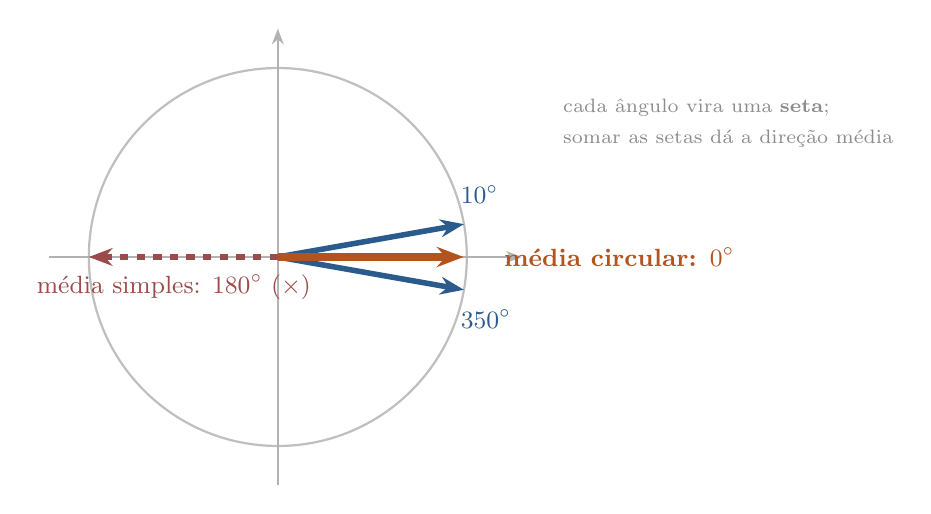
\begin{tikzpicture}[x=1cm,y=1cm]
\draw[black!25, line width=0.8pt] (0,0) circle (2.40);
\draw[daxis] (-2.90,0) -- (3.10,0); \draw[daxis] (0,-2.90) -- (0,2.90);
\draw[dblue, line width=2pt, -{Stealth[length=3mm]}] (0,0) -- (10:2.40); \node[dblue, font=\small, anchor=south west] at (2.2,0.55) {$10^{\circ}$};
\draw[dblue, line width=2pt, -{Stealth[length=3mm]}] (0,0) -- (-10:2.40); \node[dblue, font=\small, anchor=north west] at (2.2,-0.55) {$350^{\circ}$};
\draw[dorange, line width=3pt, -{Stealth[length=3.4mm]}] (0,0) -- (2.36,0); \node[dorange, font=\small\bfseries, anchor=west] at (2.75,0) {média circular: $0^{\circ}$};
\draw[dred, line width=2pt, dashed, -{Stealth[length=3mm]}] (0,0) -- (-2.40,0); \node[dred, font=\small, anchor=north] at (-1.32,-0.1) {média simples: $180^{\circ}$ ($\times$)};
\node[dsub, font=\scriptsize, anchor=west] at (3.50,1.9) {cada ângulo vira uma \textbf{seta};};\node[dsub, font=\scriptsize, anchor=west] at (3.50,1.5) {somar as setas dá a direção média};
\end{tikzpicture}
\end{document}
